\documentclass[twoside]{article}
\setlength{\oddsidemargin}{0.25 in}
\setlength{\evensidemargin}{-0.25 in}
\setlength{\topmargin}{-0.6 in}
\setlength{\textwidth}{6.5 in}
\setlength{\textheight}{8.5 in}
\setlength{\headsep}{0.75 in}
\setlength{\parindent}{0 in}
\setlength{\parskip}{0.1 in}

\usepackage{graphicx}
\usepackage{url}

%
% The following commands sets up the lecnum (lecture number)
% counter and make various numbering schemes work relative
% to the lecture number.
%
\newcounter{lecnum}
\renewcommand{\thepage}{\thelecnum-\arabic{page}}
\renewcommand{\thesection}{\thelecnum.\arabic{section}}
\renewcommand{\theequation}{\thelecnum.\arabic{equation}}
\renewcommand{\thefigure}{\thelecnum.\arabic{figure}}
\renewcommand{\thetable}{\thelecnum.\arabic{table}}
\newcommand{\dnl}{\mbox{}\par}

%
% The following macro is used to generate the header.
%
\newcommand{\lecture}[4]{
  \pagestyle{myheadings}
  \thispagestyle{plain}
  \newpage
  \setcounter{lecnum}{#1}
  \setcounter{page}{1}
  \noindent
  \begin{center}
  \framebox{
     \vbox{\vspace{2mm}
   \hbox to 6.28in { {\bf COMPSCI~630~~~Systems
                       \hfill Spring 2017} }
      \vspace{4mm}
      \hbox to 6.28in { {\Large \hfill Lecture #1: #2  \hfill} }
      \vspace{2mm}
      \hbox to 6.28in { {\it Lecturer: #3 \hfill Scribe(s): #4} }
     \vspace{2mm}}
  }
  \end{center}
  \markboth{Lecture {#1}: #2}{Lecture {#1}: #2}
  \vspace*{4mm}
}

%
% Convention for citations is authors' initials followed by the year.
% For example, to cite a paper by Leighton and Maggs you would type
% \cite{LM89}, and to cite a paper by Strassen you would type \cite{S69}.
% (To avoid bibliography problems, for now we redefine the \cite command.)
%
\renewcommand{\cite}[1]{[#1]}

% \input{epsf}

%Use this command for a figure; it puts a figure in wherever you want it.
%usage: \fig{NUMBER}{FIGURE-SIZE}{CAPTION}{FILENAME}
\newcommand{\fig}[4]{
           \vspace{0.2 in}
           \setlength{\epsfxsize}{#2}
           \centerline{\epsfbox{#4}}
           \begin{center}
           Figure \thelecnum.#1:~#3
           \end{center}
   }

% Use these for theorems, lemmas, proofs, etc.
\newtheorem{theorem}{Theorem}[lecnum]
\newtheorem{lemma}[theorem]{Lemma}
\newtheorem{proposition}[theorem]{Proposition}
\newtheorem{claim}[theorem]{Claim}
\newtheorem{corollary}[theorem]{Corollary}
\newtheorem{definition}[theorem]{Definition}
\newenvironment{proof}{{\bf Proof:}}{\hfill\rule{2mm}{2mm}}

% Some useful equation alignment commands, borrowed from TeX
\makeatletter
\def\eqalign#1{\,\vcenter{\openup\jot\m@th
 \ialign{\strut\hfil$\displaystyle{##}$&$\displaystyle{{}##}$\hfil
     \crcr#1\crcr}}\,}
\def\eqalignno#1{\displ@y \tabskip\@centering
 \halign to\displaywidth{\hfil$\displaystyle{##}$\tabskip\z@skip
   &$\displaystyle{{}##}$\hfil\tabskip\@centering
   &\llap{$##$}\tabskip\z@skip\crcr
   #1\crcr}}
\def\leqalignno#1{\displ@y \tabskip\@centering
 \halign to\displaywidth{\hfil$\displaystyle{##}$\tabskip\z@skip
   &$\displaystyle{{}##}$\hfil\tabskip\@centering
   &\kern-\displaywidth\rlap{$##$}\tabskip\displaywidth\crcr
   #1\crcr}}
\makeatother

% **** IF YOU WANT TO DEFINE ADDITIONAL MACROS FOR YOURSELF, PUT THEM HERE:



% Some general latex examples and examples making use of the
% macros follow.

\begin{document}

%FILL IN THE RIGHT INFO.
%\lecture{**LECTURE-NUMBER**}{**DATE**}{**LECTURER**}{**SCRIBE**}
\lecture{11}{Hints for Computer System Design}{Emery Berger}{Manish Motwani, Rohini Kapoor}

\section{Road to Computer System Design}
We first briefly talked about end-to-end argument discussed in previous lecture wherein we discussed that functionality that ensures whether correct transmission of data packets occurred should be implemented in the end systems rather than underlying network transmission mechanisms. For example, when we are transferring large chunk of data (BitTorrent) by splitting it into smaller chunks then we anyhow need to verify if that all the smaller chunks are received at the recipient system before we combine them. Similarly, if we are sending encrypted data then encryption and decryption functionalities are required to be implemented on sender and receiver systems. In both of these cases, we can’t rely just on underlying TCP/IP to ensure these desired functionalities. \\
Side note on encryption: Padding of encrypted data packets so as to make them equal sized (using “nonce” values)  can be done on system and not by TCP/IP or other network mechanism.  Application-level invariants must be dealt on end systems rather than transport level mechanism. \\
We then talked about Hints paper. This is different than other papers because it doesn’t describe any mathematical arguments or proofs. It is more like a collection of wisdom. Also, the paper was published in 1983 and some things have changed now but not all. The paper is describes three important things: (1) Functionality, (2) Speed and (3) Fault tolerance.   
\\
We first discussed about Fault tolerance considering the example of application crash. We discussed about what could be the possible reasons for application crash (say in iphone) and the fault tolerance mechanism employed for it. Following are some of the reasons and fault tolerance mechanisms we discussed.
\subsection{Out of memory (OOM) error}
In this, applications runs out of memory. In this case, the fault mechanism employed is to signal the application before crashing so that it can save the data. An application gets a signal for OOM from OS and is supposed to save as much as it can before it gets terminated. Sometimes, the application may need more memory to do such last minute tasks and since enough memory is not available it just gets terminated. In Java, after getting OOM signal an application can throw exception Heap out of memory but since these exceptions are objects and to raise them requires more memory hence an application may not always be able to throw it. In IOS, a signal is sent to application before completely running out of memory so that it can perform last minute tasks. In C++/ObjC, null/bad\_alloc are used to indicate OOM error. 
\subsection{Segmentation Fault (SegFault) or Access Violation (AV)}
This occurs when an application tries to access illegal memory address. For example, in C/C++ when we get null dereference or illegal pointer reference. In Java, we get uncaught exceptions for this error. (side note: Q. Can the stack trace displayed on browser of the crashed web-application be a security hazard? Ans. stack trace gives control flow and doesn’t exposes the data but one could craft inputs and flood the server to create denial of service (DOS) attack)
\subsection{Signals}
Systems use different types of signals to indicate the fault in application. For example,  SIGILL is thrown while running an arm code on x86 machine, SIGBUS is thrown when memory is not aligned in boundaries and, SIGFPE is thrown when we have floating point exception (e.g. divide by 0). \\
Unanticipated or malformed input: To address this there is a “best effort” mechanism wherein an application tries to do something useful on failure for example describing some information about inputs that led to failure. Nowadays,  systems are tested using “Fuzz testing” wherein we deliberately generate weird inputs to test if the application crashes, This is used for security testing.
\\
We then talked about Erlang (programming language used for telecommunication systems)  which is well known for designing fault tolerant systems. Fault tolerance assumes that something bad is going to happen and what useful things could be done about it. A possible fault tolerance mechanism is to save  the state (e.g. all the files and data) of the system and make the system persistent. If everything before the application got crashed was successfully saved then re-starting the application is not a major concern for the users. This is  ad-hoc form of fault localization. Building universal fault tolerance that addresses the issues completely is hard and expensive. 
\section{System Designing}
We then talked about system designing. While creating systems, one should separate normal case and worst case. Following KISS (keep it simple stupid) principle is a good idea while creating systems. Occam’s razor (similar to KISS) states that “do one thing and do it well” and it is a good idea to follow this while creating systems. These principles are described using examples of Windows API vs. Linux API wherein Windows API is like a swiss army knife which has every tool you need but using any of the tools is not a good experience.  In Windows API the function names are huge (GetCurrentDirectory vs getcwd, VirtualAlloc vs mmap). In Linux, APIs don’t get to allocate memory and a buffer of fixed size is allocated for them. In Windows API, methods have huge number of arguments unline Linux API (e.g. pthread.create method requires only two arguments in Linux API). Considering all this, why would one want to use Windows API? The only advantage of using Windows API is that it makes one system call or invokes one kernel process to do the job which leads to high performance. 
\\
Another important aspect we talked about was “plan to throw it away” or “second system effect” wherein it is often found that the second system build is more cleaner (simple) and efficient realizing the shortcomings of the first system. For example, Unix was created after Multics, C\# was created after Java. We discussed more about it by talking about how parameters were passed in function arguments in JAVA. Primitive types(like int) are passed by value in function calls. This means that when those variables are altered in the function, these changes will not be seen in the calling function, they are referred to as unboxed values.\\ Objects(such as Integers), on the other hand, are passed by reference, and are boxed variables. Java relied on programmer to know this distinction. C\#, on the other hand, does this boxing/unboxing automatically, and hence has learnt by the mistakes of JAVA. The later versions of Java incorporate the advances made in C\# We also talked about how JAVA failed in its original mission. Java was first rendered to be used in Embedded programming, and then later to make websites. Javascript is also an example of the second system effect. It learnt from the mistakes of Java, and is not being used for website development. Another example, we considered was of Chorme which was created after firefox which crashes completely when multiple tabs are opened. In Chrome each tab is an isolated process so if one process crashes others are not affected (another example of ad-hoc fault tolerance).  We briefly talked about Replication which is useful for fault tolerance as the replicas can be used to restore the state of the system. 
\\
We then shifted our discussion to Speed which is necessary but not sufficient characteristics of the system. We talked about Quantization wherein we create bins of fixed size (“quantize”) in the memory so as to minimize the storage and also to increase the processing  speed of the applications. 
\\
We then talk about how a system deals with excessive load. Excessive load in the system leads to non-responsiveness because of thrashing, where the system does more work in switching between tasks than the work. A system, thus, gets rid of extra load in case of excessive loads. It can either deny entry to an incoming task(admission control) or kill a process within. The latter is called load shedding, and it allows the system to kill tasks that consume too much memory or take large times to execute. This is why systems prefer Atomicity transactions, so that no major information is lost during load shedding.

\begin{figure}[!h]
    \centering
    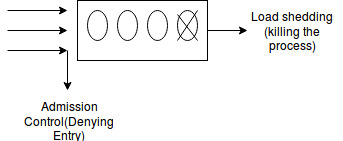
\includegraphics{Diagram.jpg}
    \caption{Load Shedding}
    \label{Load Shedding}
\end{figure}

For hints, the system tries to optimize for common case, for example, in case of branch prediction it takes advantage of spatial locality and puts more probable ones together. We do not cache while I/O streaming due to the lack of temporal cache, or for the random function due to the lack of spatial locality.\\
We discussed the use of background threads, and revisited the concepts of concurrent Garbage collector vs stop the world garbage collector. When we load a webpage, usually, the images are loaded from some other sources. This is done using background threads, so as to keep this task separate from the thread loading the other contents. These images are stored on disk for future use.
\subsection{Caching}
We discussed the various ways for caching. We start with memoization, where if we have a function f(x)->v, which takes long time to compute, we store it in a table, and use it for future use. We can only do this if the function f(x) is side effect free, ie., it is deterministic and does not change the global variables. The next time the function is used, instead of recalculating the value, we directly retrieve it from the lookup table. This is similar to what is done with Dynamic programming. Fibonacci series is an example for this technique. If we recompute the values everytime, the complexity becomes exponential. With memoization, we can do it in linear time, by storing the values in a table. \\
Amortization is a concept where the cost is paid by spreading over multiple computations. An example is loading a webpage one at a time as and when required rather than loading the entire website. \\
An example for this is expanding the size of the buffer. We can increase the size one at a time as elements are added. In that case the complexity is O(n2). One other way would be to increase by 10 everytime the buffer is full. The complexity would still be O(n2), with a lesser value for n. The optimal solution to this problem is the double the size every time the buffer gets full. This leads to a complexity of O(n). This resembles the ski-rental problem which states that never pay more than double.\\
Piggybacking on the other hand refers to the concept that while the system is doing one thing, it should do something else also. This is done to save cost. For example, during image transfer, also request for the next webpage.

\end{document}